\chapter{Jeu sous forme normale}

\section{Introduction et Informations Pratiques}

\begin{itemize}
    \item \textbf{Enseignant :} Philippe BICH (bich@univ-paris1.fr)
    \item \textbf{Crédits :} 5 ECTS (pour Théorie des Jeux 1-2)
    \item \textbf{Méthode :} Cours magistral et résolution de problèmes.
    \item \textbf{Prérequis :} Analyse et bases de probabilités.
    \item \textbf{Références :}
        \begin{enumerate}
            \item "Game theory" - Maschler, Solan, Zamir
            \item "Bases mathématiques de la théorie des jeux" - Sorin, Laraki, Renault
        \end{enumerate}
    \item \textbf{Évaluation :} Présence, exercices des slides (avec bonus pour les exercices étoffés *) et examen final reprenant des questions similaires. \textbf{Attention :} La qualité de l'argumentation et du raisonnement compte autant, sinon plus, que le résultat du calcul.
\end{itemize}

\section{Concepts Introductifs}
La théorie des jeux analyse les situations où le comportement optimal d'un individu dépend des choix des autres. C'est un domaine interdisciplinaire majeur.

\begin{itemize}
    \item \textbf{Économie :} Prix d'Apple, enchères.
    \item \textbf{Finance :} Stratégies de portefeuille, détermination du prix d'instruments financiers.
    \item \textbf{Biologie :} Stratégies coopératives des espèces, évolution.
    \item \textbf{Politique :} Armement nucléaire, votes, grèves.
    \item \textbf{Réseaux :} Décision de créer un lien sur un réseau social, transmission d'information ou de publicité.
    \item \textbf{Mathématiques \& Mean Field Games :} Analyse de situations où le comportement dépend de la moyenne d'un grand nombre de personnes (ex: choix d'un chemin optimal dans le trafic, choix de localisation).
\end{itemize}

\paragraph{Contexte Académique :}
La théorie des jeux est un pilier de la recherche moderne. \textbf{Plus d'une douzaine de prix Nobel} ont été décernés à des théoriciens des jeux, dont beaucoup sont mathématiciens (plus que de simples économistes). On citera notamment \textbf{John Nash}, popularisé par le film "Un homme d'exception" (A Beautiful Mind).

\paragraph{Nuances Importantes :}
\begin{itemize}
    \item \textbf{Modèle de Schelling (Ségrégation)} :
Ce modèle illustre comment des préférences individuelles faibles pour la mixité peuvent mener à une ségrégation totale. 
\begin{itemize}
    \item Une grille où chaque cellule est occupée par un agent de type A ou B.
    \item Un agent est satisfait si au moins un certain pourcentage de ses voisins est de son type.
    \item Sinon, il déménage vers la cellule vide la plus proche qui le satisfait.
\end{itemize}

\begin{center}
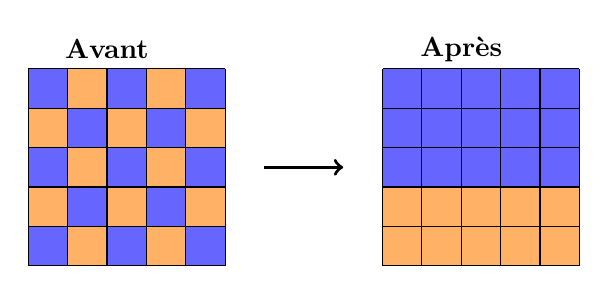
\begin{tikzpicture}[scale=0.5]
    % Before grid (checkerboard pattern)
    \node at (2, 5.5) {\textbf{Avant}};
    % Row 0
    \fill[blue!60] (0,0) rectangle (1,1); \fill[orange!60] (1,0) rectangle (2,1);
    \fill[blue!60] (2,0) rectangle (3,1); \fill[orange!60] (3,0) rectangle (4,1);
    \fill[blue!60] (4,0) rectangle (5,1);
    % Row 1
    \fill[orange!60] (0,1) rectangle (1,2); \fill[blue!60] (1,1) rectangle (2,2);
    \fill[orange!60] (2,1) rectangle (3,2); \fill[blue!60] (3,1) rectangle (4,2);
    \fill[orange!60] (4,1) rectangle (5,2);
    % Row 2
    \fill[blue!60] (0,2) rectangle (1,3); \fill[orange!60] (1,2) rectangle (2,3);
    \fill[blue!60] (2,2) rectangle (3,3); \fill[orange!60] (3,2) rectangle (4,3);
    \fill[blue!60] (4,2) rectangle (5,3);
    % Row 3
    \fill[orange!60] (0,3) rectangle (1,4); \fill[blue!60] (1,3) rectangle (2,4);
    \fill[orange!60] (2,3) rectangle (3,4); \fill[blue!60] (3,3) rectangle (4,4);
    \fill[orange!60] (4,3) rectangle (5,4);
    % Row 4
    \fill[blue!60] (0,4) rectangle (1,5); \fill[orange!60] (1,4) rectangle (2,5);
    \fill[blue!60] (2,4) rectangle (3,5); \fill[orange!60] (3,4) rectangle (4,5);
    \fill[blue!60] (4,4) rectangle (5,5);
    % Grid lines
    \draw (0,0) grid (5,5);
    
    % Arrow
    \draw[->, very thick] (6, 2.5) -- (8, 2.5);
    
    % After grid (segregated)
    \node at (11, 5.5) {\textbf{Après}};
    % Bottom rows (orange)
    \fill[orange!60] (9,0) rectangle (14,2);
    % Top rows (blue)
    \fill[blue!60] (9,2) rectangle (14,5);
    % Grid lines
    \draw (9,0) grid (14,5);
\end{tikzpicture}
\captionof{figure}{Modèle de Schelling : ségrégation émergente.}
\end{center}
\end{itemize}

\section{Jeu sous forme normale}

\subsection{Définitions}
\begin{definition}
Un \textbf{jeu sous forme normale} est un triplet $(N, (X_i)_{i \in N}, (u_i)_{i \in N})$ où :
\begin{itemize}
    \item $N$ est l'ensemble des joueurs.
    \item $X_i$ est l'ensemble des actions du joueur $i \in N$.
    \item $u_i: X \rightarrow \mathbb{R}$ est la fonction de gain.
    \item $X = \prod_{i \in N} X_i$ représente l'ensemble des \textbf{profils d'actions}. Un profil est une liste $x = (x_1, x_2, \dots, x_n)$ contenant une action pour chaque joueur.
\end{itemize}
\end{definition}

\subsection{Exemples Célèbres}

\begin{enumerate}
    \item \textbf{Jeu de coordination :}
    \begin{center}
    \begin{tabular}{c|c|c}
     & A & B \\ \hline
    A & (1, 1) & (0, 0) \\ \hline
    B & (0, 0) & (2, 2)
    \end{tabular}
    \end{center}

    \item \textbf{Jeu de la poule mouillée (Chicken Game / Hawk-Dove) :}
    \begin{center}
    \begin{tabular}{c|c|c}
     & Dévier & Foncer \\ \hline
    Dévier & (0, 0) & (-1, 1) \\ \hline
    Foncer & (1, -1) & (-10, -10)
    \end{tabular}
    \end{center}

    \item \textbf{Jeu des pièces de monnaie (Matching Pennies) :}
    \begin{center}
    \begin{tabular}{c|c|c}
     & Pile & Face \\ \hline
    Pile & (1, -1) & (-1, 1) \\ \hline
    Face & (-1, 1) & (1, -1)
    \end{tabular}
    \end{center}

    \item \textbf{Dilemme du prisonnier :}
    \begin{center}
    \begin{tabular}{c|c|c}
     & Ne pas confesser & Confesser \\ \hline
    Ne pas confesser & (-1, -1) & (-10, 0) \\ \hline
    Confesser & (0, -10) & (-5, -5)
    \end{tabular}
    \end{center}

    \item \textbf{Guess two-third of the average :}
    Ce jeu illustre que votre stratégie optimale dépend de votre capacité à deviner le niveau de rationalité des autres joueurs.
\end{enumerate}

\subsection{Exemples de jeux continus}

\paragraph{Enchère au premier prix}
$N = \{1, 2\}$, $X_1 = X_2 = [0, +\infty[$. Valeurs $v_1 = 1M, v_2 = 1.1M$.
$$u_i(x_i, x_j) = \begin{cases} v_i - x_i & \text{si } x_i > x_j \\ \frac{v_i - x_i}{2} & \text{si } x_i = x_j \\ 0 & \text{sinon} \end{cases}$$

\begin{center}
\begin{tikzpicture}[scale=0.8]
    \draw[->] (0,0) -- (5,0) node[right] {$x_1$};
    \draw[->] (0,-0.5) -- (0,3) node[above] {$u_1$};
    % u_1 = 0 for x_1 < x_2
    \draw[thick, blue] (0,0) -- (2,0);
    % Discontinuity at x_1 = x_2
    \fill[blue] (2,0) circle (2pt);
    \draw[blue, dashed] (2,0) -- (2,1.5);
    \fill[white] (2,1.5) circle (2pt);
    \draw[blue] (2,1.5) circle (2pt);
    % u_1 = v_1 - x_1 for x_1 > x_2
    \draw[thick, blue] (2,1.5) -- (4,0.5);
    % Labels
    \node[below] at (2,0) {$x_2$};
    \node[left] at (0,1.5) {$v_1 - x_2$};
    \draw[dashed, gray] (0,1.5) -- (2,1.5);
\end{tikzpicture}
\captionof{figure}{Gain $u_1(x_1)$ pour $x_2$ fixé : discontinuité en $x_1 = x_2$.}
\end{center}
\begin{figureexplanation}
Ce graphique illustre la discontinuité du gain dans une enchère au premier prix.
\begin{itemize}
    \item Si le joueur joue $x_1 < x_2$, il perd et gagne 0.
    \item S'il joue $x_1 = x_2$, il partage le gain à 50\% (point blanc/cercle).
    \item S'il joue $x_1 > x_2$ (même de très peu), il gagne tout le marché (saut brutal du gain).
\end{itemize}
Cette discontinuité empêche l'application directe du théorème de Nash (qui requiert des fonctions de gain continues).
\end{figureexplanation}
\paragraph{Enchère au second prix (Vickrey)}
Deux joueurs $i=1,2$ avec des valorisations $v_i$. Ils soumettent des offres $x_i \ge 0$. Le gagnant paie l'offre du perdant.
\[
u_1(x_1, x_2) = 
\begin{cases} 
v_1 - x_2 & \text{si } x_1 > x_2 \\
\frac{v_1 - x_2}{2} & \text{si } x_1 = x_2 \\
0 & \text{si } x_1 < x_2
\end{cases}
\]

\section{Exercices}

\begin{exemple}[All pay auction]
Tous les enchérisseurs paient leur offre, que l'objet soit remporté ou non. Le plus offrant remporte l'objet.
\begin{itemize}
    \item \textbf{Mécanisme :} Chaque joueur soumet une offre $x_i \ge 0$.
    \item \textbf{Fonction de gain :} Pour le joueur $i$, avec une valorisation $v_i$ :
    \[ u_i(x_i, x_{-i}) = \begin{cases} v_i - x_i & \text{si } x_i > x_j \quad \forall j \neq i \\ -x_i & \text{si } x_i < \max(x_{-i}) \end{cases} \]
    (En cas d'égalité pour l'offre la plus élevée, le gain peut être partagé).
\end{itemize}
\end{exemple}

\begin{exemple}[Ice-cream sellers (Hotelling)]
\textbf{Consigne :} Deux vendeurs se placent sur l'intervalle $[0, 1]$. Les clients sont répartis uniformément et vont au vendeur le plus proche.
\begin{enumerate}
    \item Écrire formellement les fonctions de gain.
    \item Tracer $u_1(x_1, x_2)$ pour une valeur fixée $x_2 < 1$.
\end{enumerate}

\paragraph{Correction :}
\begin{enumerate}
    \item Les clients choisissent le vendeur le plus proche. Le client "indifférent" se situe au milieu des deux vendeurs, soit en $m = \frac{x_1 + x_2}{2}$.
   Si $x_1 < x_2$, le Vendeur 1 capture tous les clients de $[0, m]$. Son gain (part de marché) est :
   $$u_1(x_1, x_2) = \frac{x_1 + x_2}{2}$$
   Si $x_1 > x_2$, le Vendeur 1 capture les clients de $[m, 1]$. Son gain est :
   $$u_1(x_1, x_2) = 1 - \frac{x_1 + x_2}{2}$$
   Si $x_1 = x_2$, ils partagent le marché : $u_1 = 1/2$.

    \item Pour $x_2$ fixé (disons $x_2 = 0.7$), voici l'allure de $u_1(x_1)$ :
\begin{center}
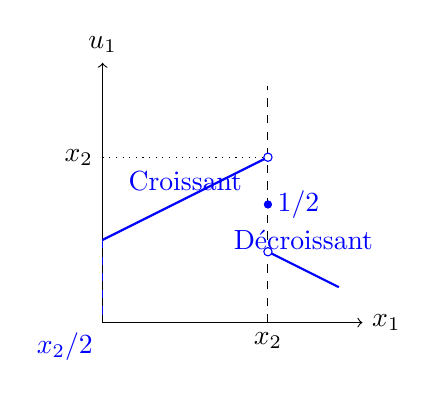
\begin{tikzpicture}[scale=3]
    \draw[->] (0,0) -- (1.1,0) node[right] {$x_1$};
    \draw[->] (0,0) -- (0,1.1) node[above] {$u_1$};
    \node[below] at (0.7,0) {$x_2$};
    \draw[dashed] (0.7,0) -- (0.7,1);
    
    % First part: increasing
    \draw[thick, blue] (0,0.35) -- (0.7,0.7); % Starts at 0.7/2 = 0.35, ends at 1.4/2 = 0.7
    \draw[dashed, blue] (0,0.35) -- (0,0) node[below left] {$x_2/2$};
    
    % Point at x2
    \fill[white] (0.7,0.7) circle (0.5pt);
    \draw[blue] (0.7,0.7) circle (0.5pt);
    
    \fill[blue] (0.7,0.5) circle (0.5pt) node[right] {1/2}; % At x1=x2
    
    % Second part: decreasing
    \draw[thick, blue] (0.7,0.3) -- (1,0.15); % Starts at 1 - 1.4/2 = 0.3, ends at 1 - 1.7/2? No.
    % Formula x1 > x2: 1 - (x1+x2)/2.
    % At x1 -> x2+, u1 -> 1 - x2 = 0.3.
    % At x1 = 1, u1 = 1 - (1+0.7)/2 = 1 - 0.85 = 0.15.
    
    \fill[white] (0.7,0.3) circle (0.5pt);
    \draw[blue] (0.7,0.3) circle (0.5pt);
    
    \draw[dotted] (0,0.7) -- (0.7,0.7) node[left] at (0,0.7) {$x_2$}; 
    
    \node[blue] at (0.35, 0.6) {Croissant};
    \node[blue] at (0.85, 0.35) {Décroissant};
\end{tikzpicture}
\end{center}
Le maximum est atteint juste "avant" $x_2$ (pour prendre tout le marché gauche). À l'équilibre, les deux se placent au centre ($1/2$).
\end{enumerate}
\end{exemple}
